\chapter{Architectural Design}
\section{Overview: High-level components and their interaction}
The eMall system is composed by a 3-tier architecture. It's software application architecture that organizes applications into three logical tiers: the presentation tier, or user interface; the application tier, where data is processed; and the data tier, where the data associated with the application is stored and managed.
\begin{figure}[H]
    \centering
    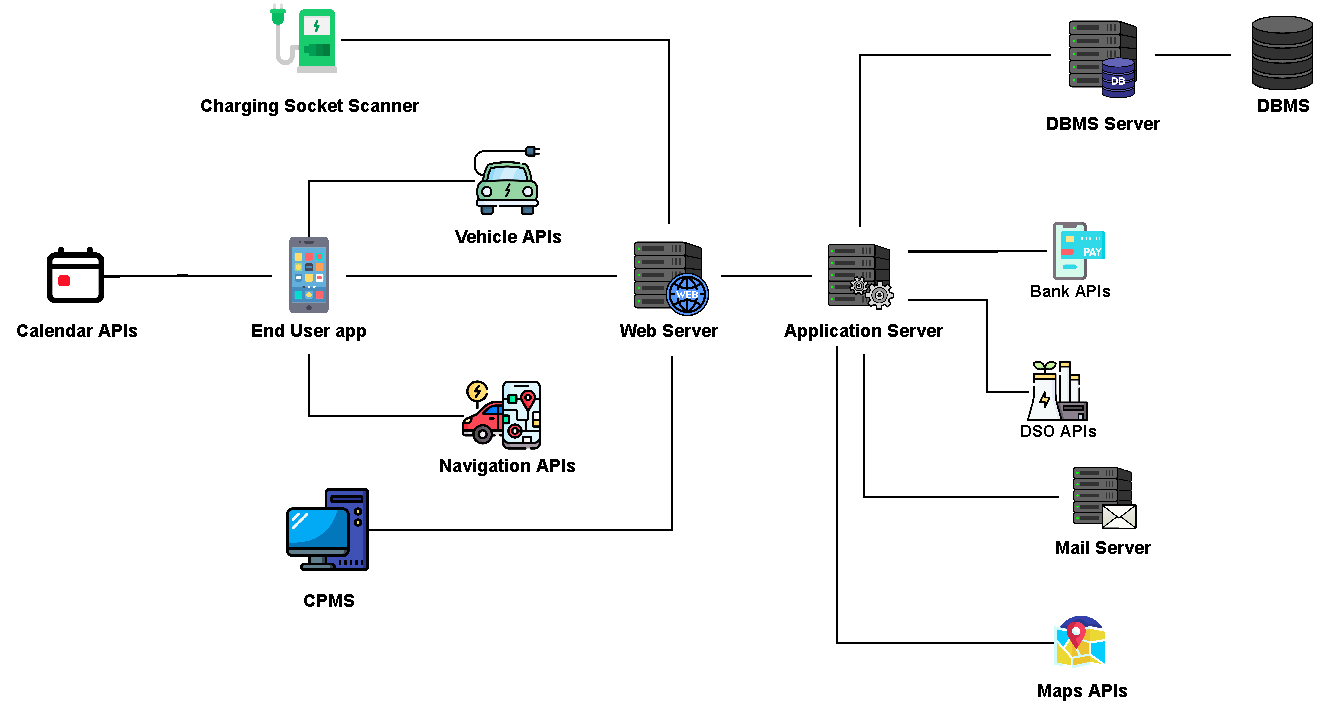
\includegraphics[width=\textwidth]{images/3tier.pdf}
    \caption{Overview eMall architecture}
    \label{fig:eMallArchitecture}
\end{figure}
The architecture of the eMall system consists of two macro areas: client-side and server-side.
\subsubsection{Client side}
On the client side, we note the mobile application of the end users, the web application (CPMS) of the CPOs and the charging socket scanner:
\begin{itemize}
    \item \textbf{End user app}: user-friendly mobile application that allows end users to manage the charging process of their electric vehicles from scratch.\\
    The choice of a mobile application is due to the fact that is easily to interact with the navigation and calendar system running on the same device and, moreover, interact with some vehicles APIs.\\
    It offers various functionalities:
    \begin{itemize}
        \item Access to electric vehicle information (charge level) and user information (personal calendar).
        \item Access to geolocation APIs that allow the identification of charging stations nearby.
        \item Selecting a station based on one's preferences and needs.
        \item Booking of a charging station at a specific timeslot.
        \item Management of start and stop of a charge.
    \end{itemize}
    \item \textbf{CPMS}: web application for CPOs to manage their charging stations. \\
    In particular a web application sufficies because the CPMS has not to communicate with a specfic CPO device or something similar.
    Specifically:
    \begin{itemize}
        \item Purchasing energy from different DSOs.
        \item Setting different special offers.
        \item Displaying battery status.
        \item Monitoring the status of own charging stations (internal and external status).
    \end{itemize}
    \item \textbf{Charging Socket Scanner}: a simple QR-Code scanner installed on each charging socket. It allows:
    \begin{itemize}
        \item Scanning the QR-Code of a user.
        \item Connection to the eMall server, sending the code to verify that a particular end user has a valid booking.
        \item Enabling charging.
    \end{itemize}
\end{itemize}
\subsubsection{Server side}
On the server side, there is an infrastructure enabling the communication of the entire system, realised by various components:
\begin{itemize}
    \item \textbf{Application Server}: server on which all the application logic resides: in addition to this, it also communicates with the Mail Server and the DBMS Server. It's also responsible for managing bank APIs to allow the system to substract end user money after a charge and for managing DSO APIs, that are useful for CPO to buy energy.
    \item \textbf{Web Server}: server that enables communication via HTTP with the various clients listed above and acts as middleware between front-end and back-end.
    \item \textbf{Mail Server}: mail server that takes care of sending e-mails (via the SMTP protocol) to the end user to confirm registration.
    \item \textbf{DBMS Server}: server that communicates with the database engine to manage, store and request all data related to the eMall system.
    
\end{itemize}
\section{Component view}
\subsection{High level view}
The component diagram reported below (Figure \ref{fig:ComponentGen}) depicts the system components and interfaces from an high level point of view. The \textbf{eMall server} component will be detailed in the following sections.
\begin{figure}[H]
    \centering
    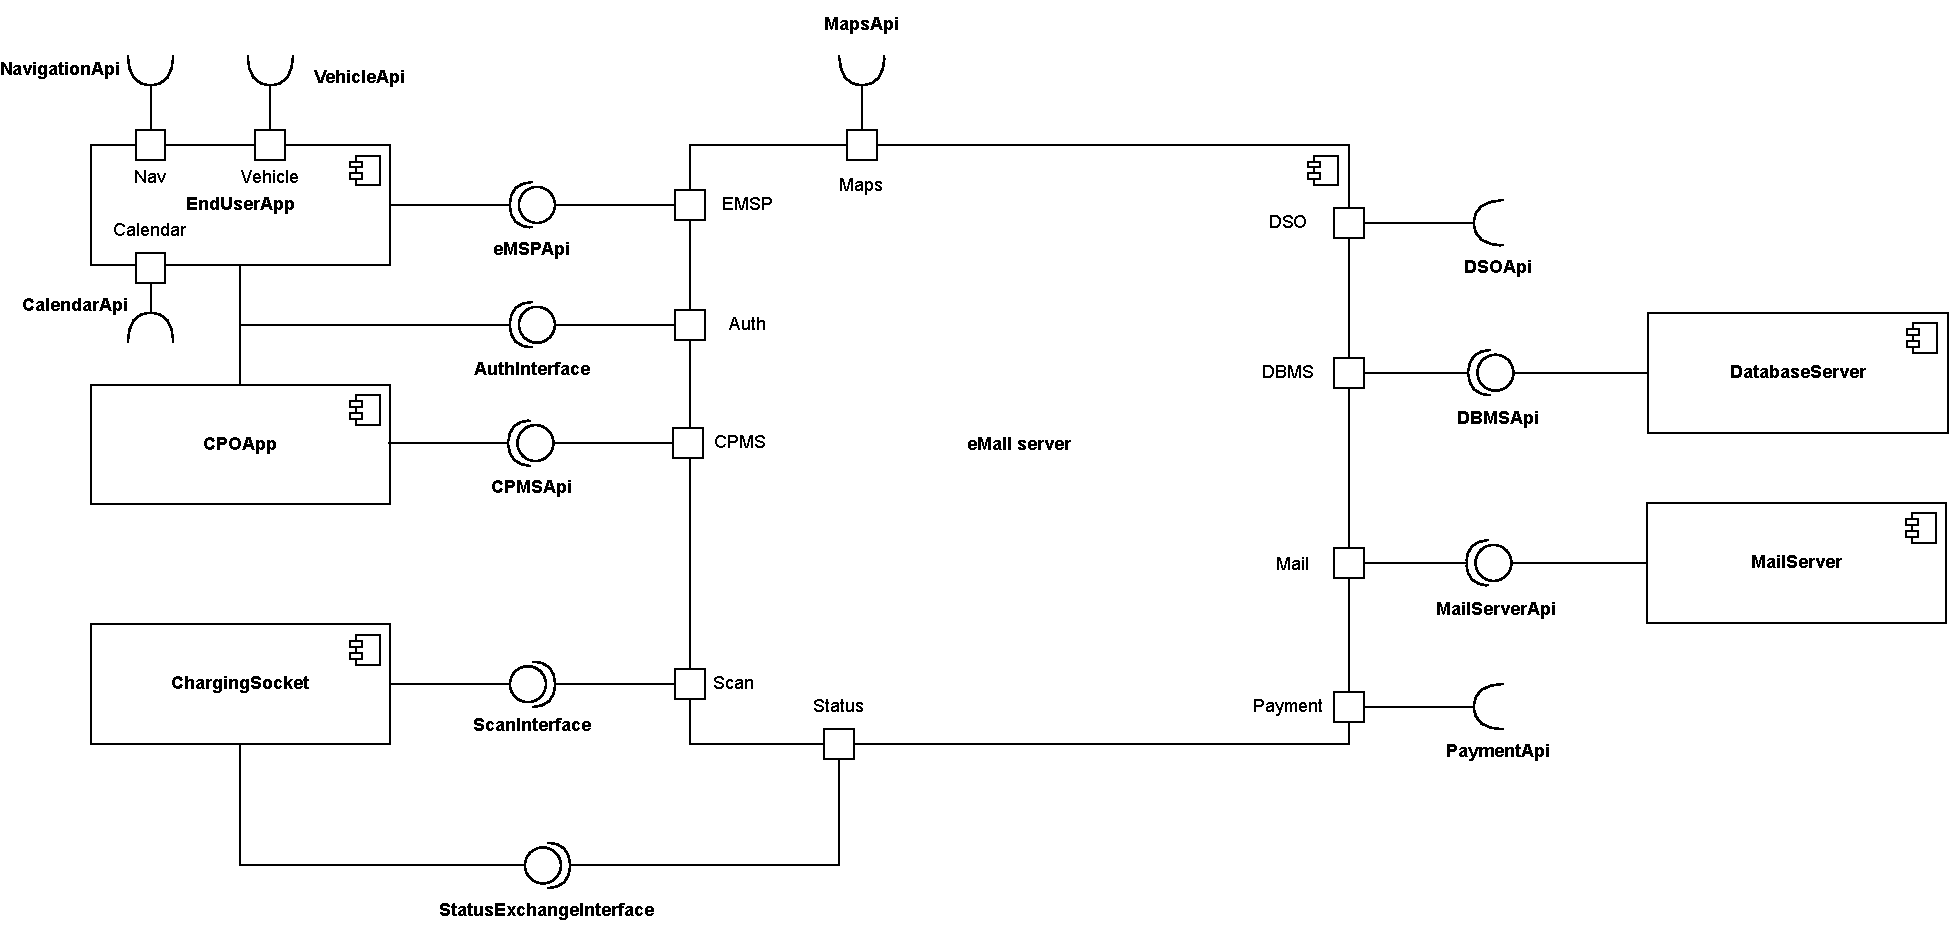
\includegraphics[width=\textwidth]{images/ComponentGenerico.pdf}
    \caption{High level component description.}
    \label{fig:ComponentGen}
\end{figure}
\begin{itemize}
    \item \textbf{eMall server}: represents the core of the eMall system, this component contains all the logic that enables the system to process and exchange information between the various systems connected to it. More specifically the eMall server provides interfaces to both, the client and the server side. This component is detailed in Figure \ref{fig:ComponentSpec}.
    \item \textbf{EndUserApp}: represents the mobile application installed on the users' devices. Through authentication (\textbf{AuthInterface}) allows access to all the features offered by the system through the \textbf{eMSPApi}.
    \item \textbf{CPOApp}: represents the web application available for the cpos. Through authentication (\textbf{AuthInterface}) allows access to all the features offered by the system through the \textbf{CPMSApi}.
    \item \textbf{ChargingSocket}: represents the charging socket, that, through the \textbf{ScanInterface} can exchange data relative to the QRCodes scanning process, while through the \textbf{StatusExchangeInterface} can exchange data relative to the status of the socket.
    \item \textbf{DatabaseServer}: represents the DBMS, this component provides to the eMall server, through the \textbf{DBMSApi}, the access to de persistent data saved in the database.
    \item \textbf{MailServer}: represents the mail server, this component provides to the eMall server, through the \textbf{MailServerApi}, all the features relative to the mail exchanging process.
\end{itemize}
\subsection{eMall server detailed view}
\begin{figure}[H]
    \centering
    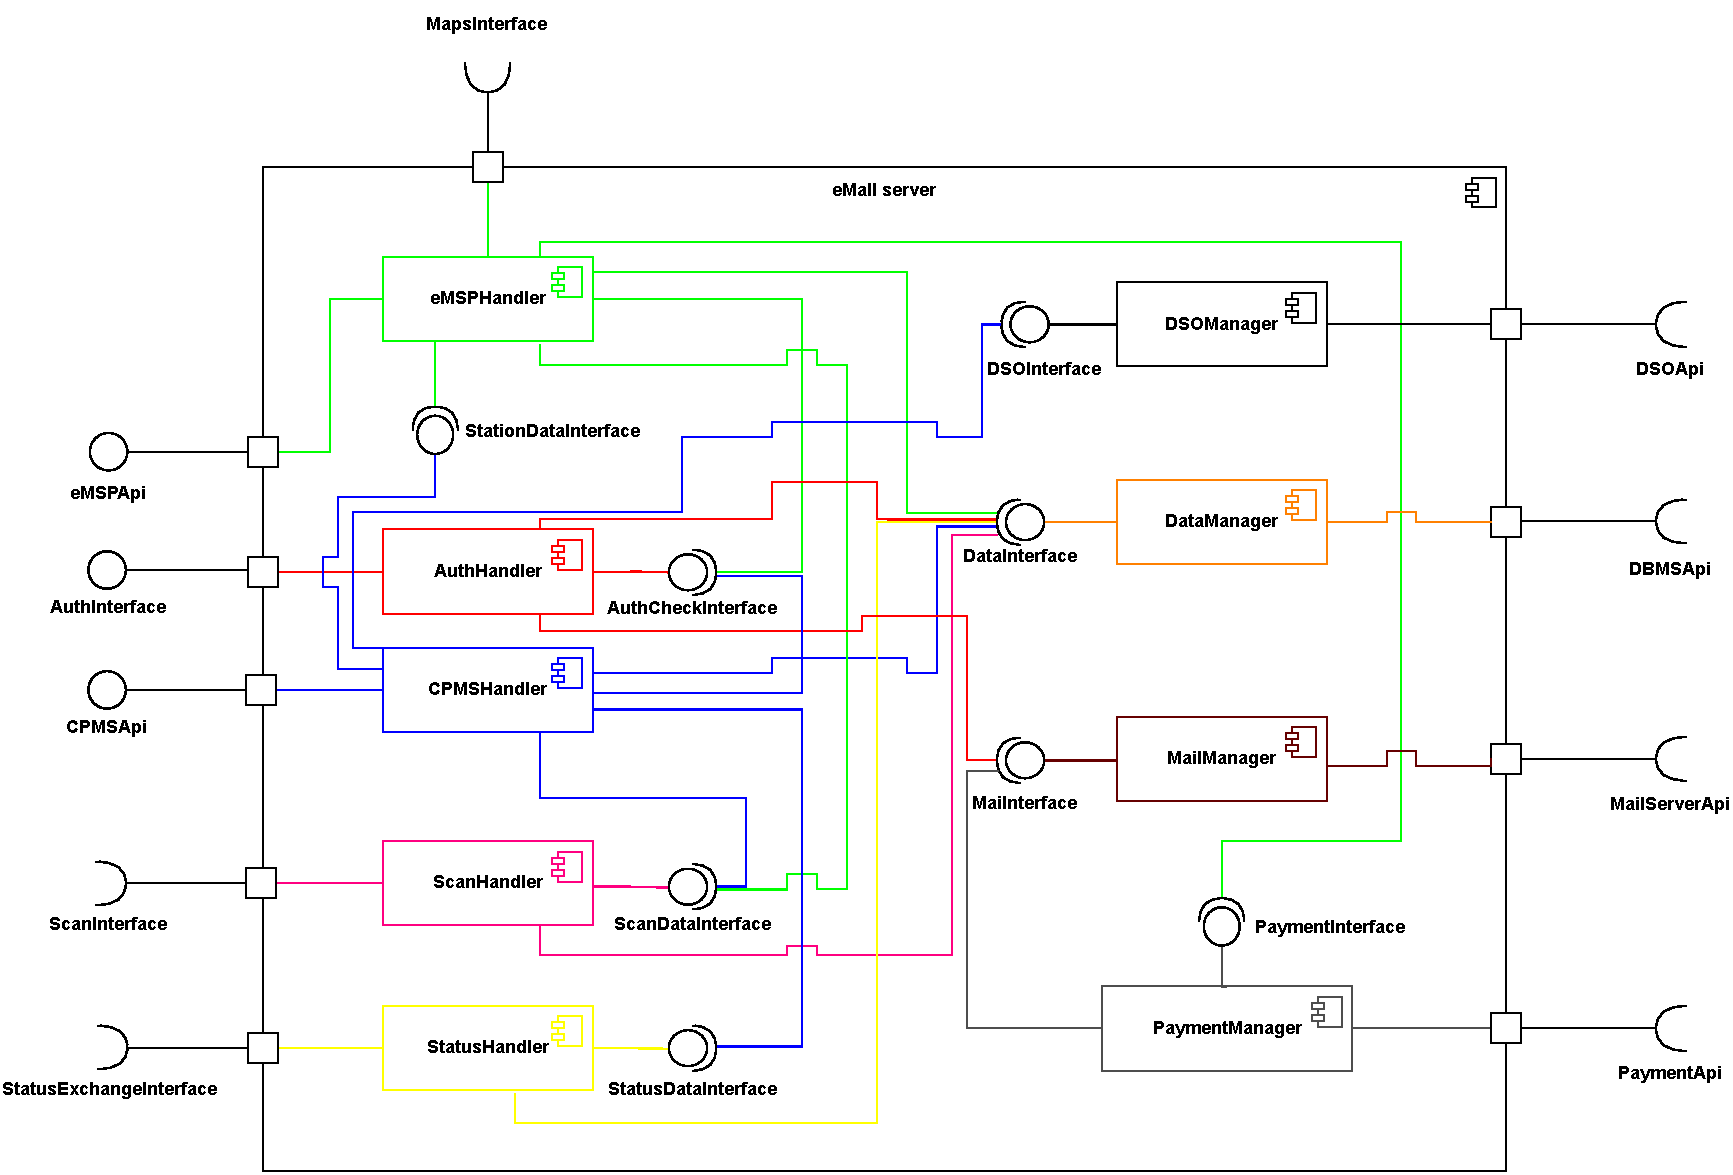
\includegraphics[width=\textwidth]{images/ComponentSpecifico.pdf}
    \caption{eMall server component diagram.}
    \label{fig:ComponentSpec}
\end{figure}
\begin{itemize}
    \item \textbf{eMSPHandler}: handles all the functionalities offered in the eMSP, for example it handles the bookings creation / deletion, view all the charging stations and charging process managment. More specifically it interfaces with the CPMS through the \textbf{StationDataInterface} to get the data regarding the charging stations and their status. The \textbf{ScanDataInterface} is used to deal with the designed charging socket, while the \textbf{AuthCheckInterface} is needed to check the authorization on all the eMSP operations. The interaction with the PaymentManager through the \textbf{PaymentInterface} is usefull to allow the user to pay for a charge. The \textbf{MapsApi} are used by the component to satisfy the charging station search requests filtering by position.Finally we have the interaction with the DBMS through the \textbf{DataInterface}, this interface is used almost by all the components because is the only access point to the persistent data.
    \item \textbf{AuthHandler} handles logins and registration from users and CPOs, it also offers an interface \textbf{AuthCheckInterface} to allow other component to check if an operation is authorized. The interface with the mail server (\textbf{MailInterface}) is used to manage the confirmation e-mails, while the \textbf{DataInterface} is used to check the credentials correctness.
    \item \textbf{CPMSHandler} it handles, similarly to the eMSPHandler, all the functionalities offered to the CPO. The \textbf{DataInterface} is used to access to the persistent data. The \textbf{ScanDataInterface} and the \textbf{StatusDataInterface} are used to monitor the sockets, while the \textbf{AuthCheckInterface} is used with the same purpose as for the eMSPHandler. The last interface to consider is the \textbf{DSOInterface} which allow the CPMS to deals with the DSOs Api.
    \item \textbf{ScanHandler} handles all the actions relative to the scanning function provided by the charging sockets, and expose an interface (\textbf{ScanDataInterface}) to allow the access to the scans data, for example to check a QRCode. This component is further detailed in figure \ref{fig:scan_comp}.
    \item \textbf{StatusHandler} handles the status updates of the charging sockets. Its job is to provide an interface (\textbf{StatusDataInterface}) for other components to access the data in the various sockets.
    \item \textbf{DataManager} handles all the accesses to the persistent data saved on the DB, it is used by almost all the components that need the data access.
    \item \textbf{MailManager} handles the access to the mail server, it provides an interface (\textbf{MailInterface}) that allows the components to interact with the mail server.
    \item \textbf{PaymentManager} handles user payment requests and forwards them to the banking system via the external \textbf{PaymentApi}. it also interacts with the MailServer (\textbf{MailInterface}) to send receipts to users.
    \item \textbf{DSOManager} handles the interactions between the CPMS and the DSO through an external api, to allow this the component provides a \textbf{DSOInterface}.
\end{itemize}
\subsection{Scan component view}
\begin{figure}[H]
    \centering
    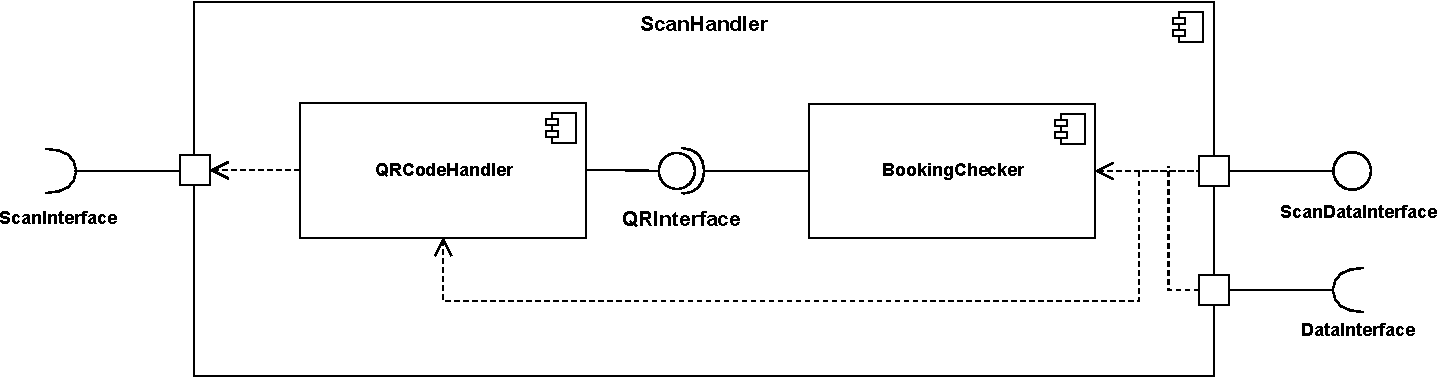
\includegraphics[width=\textwidth]{images/ScanComponent.pdf}
    \caption{Scan component view.}
    \label{fig:scan_comp}
\end{figure}
\begin{itemize}
    \item \textbf{QRCodeHandler}: handles the Scan requests, interprets them and provides the data via the interface \textbf{QRInterface}.
    \item \textbf{BookingChecker}: is the component which aim is to check if a code matches with a booking code. This is made by exploiting the two interfaces \textbf{DataInterface} and \textbf{ScanDataInterface}.
\end{itemize}
\subsection{Auth component view}
\begin{figure}[H]
    \centering
    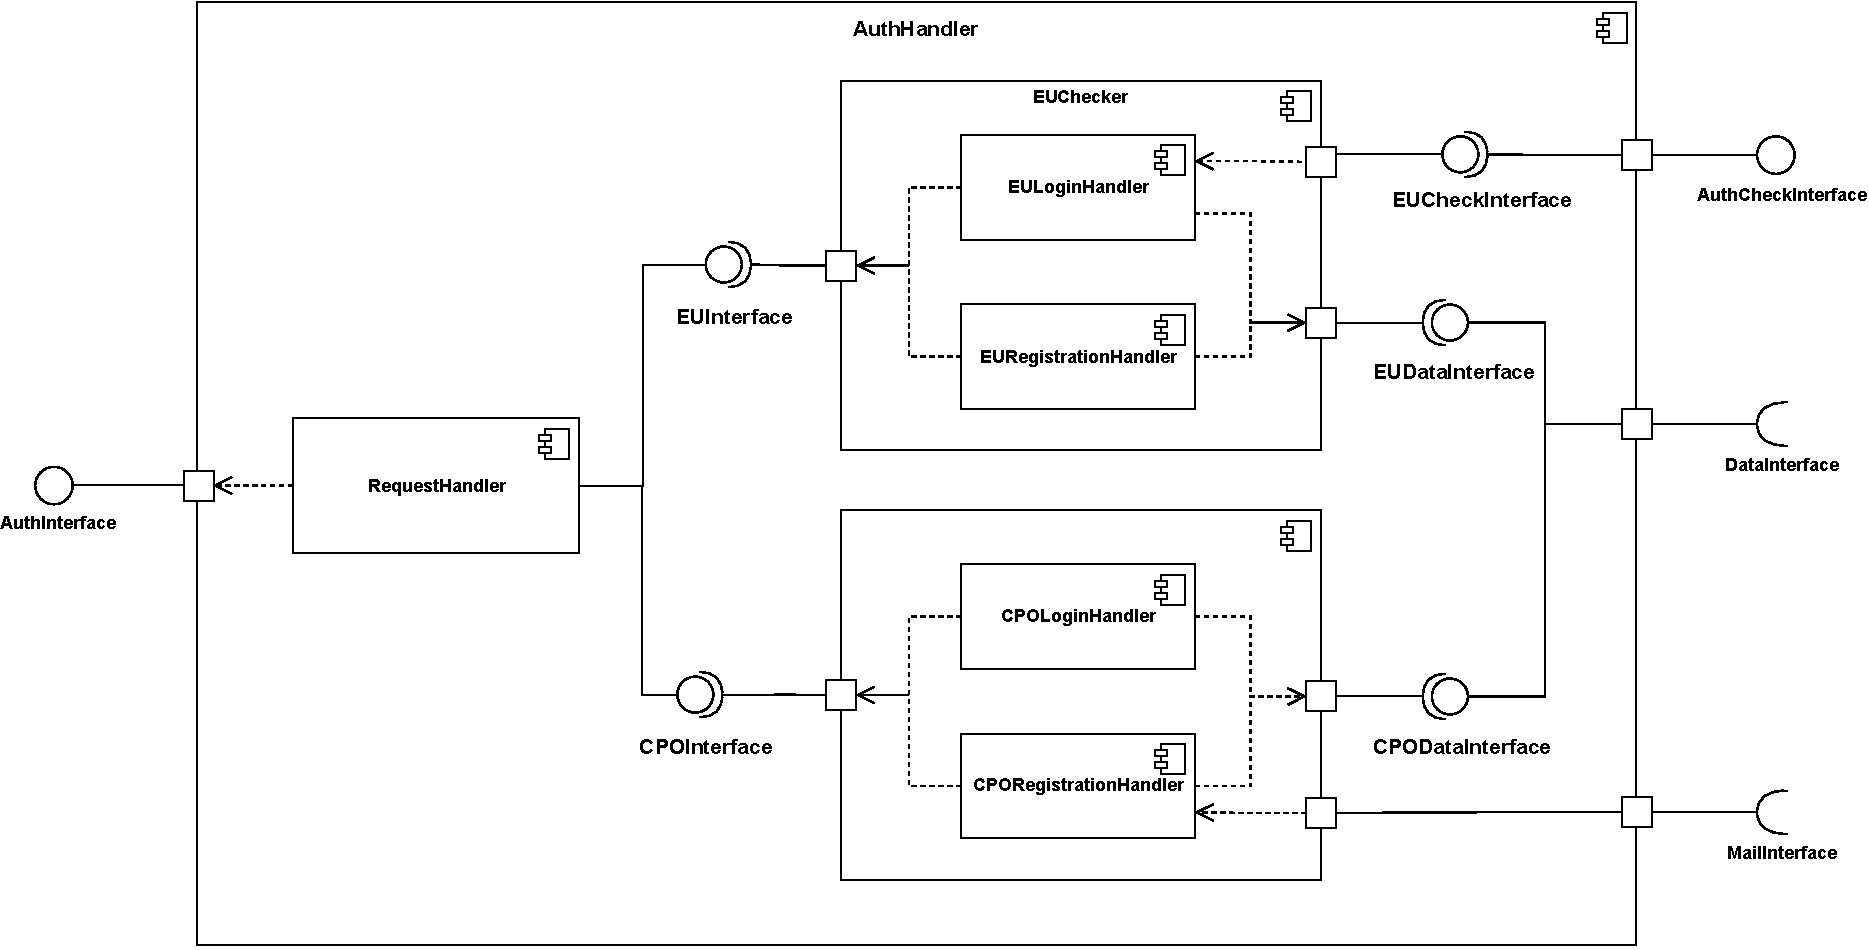
\includegraphics[width=\textwidth]{images/AuthComponent.pdf}
    \caption{Auth component view.}
    \label{fig:auth_comp}
\end{figure}
\begin{itemize}
    \item \textbf{RequestHandler}: this component handles the requests, and it acts like a router sorting requests between users' requests and CPOs' requests.
    \item \textbf{EULoginHandler}: handles the login requests made by the users.
    \item \textbf{EURegistrationHandler}: handles the registration requests made by the users. The \textbf{EUCheckInterface} allows an external component to verify the authorization of an operation.
    \item \textbf{CPOLoginHandler}: handles the login requests made by the CPOs.
    \item \textbf{CPORegistrationHandler}: handles the registration requests made by the CPOs. The \textbf{MailInterface} is used to send confirmation e-mails.
\end{itemize}
\section{Deployment View}
\begin{figure}[H]
    \centering
    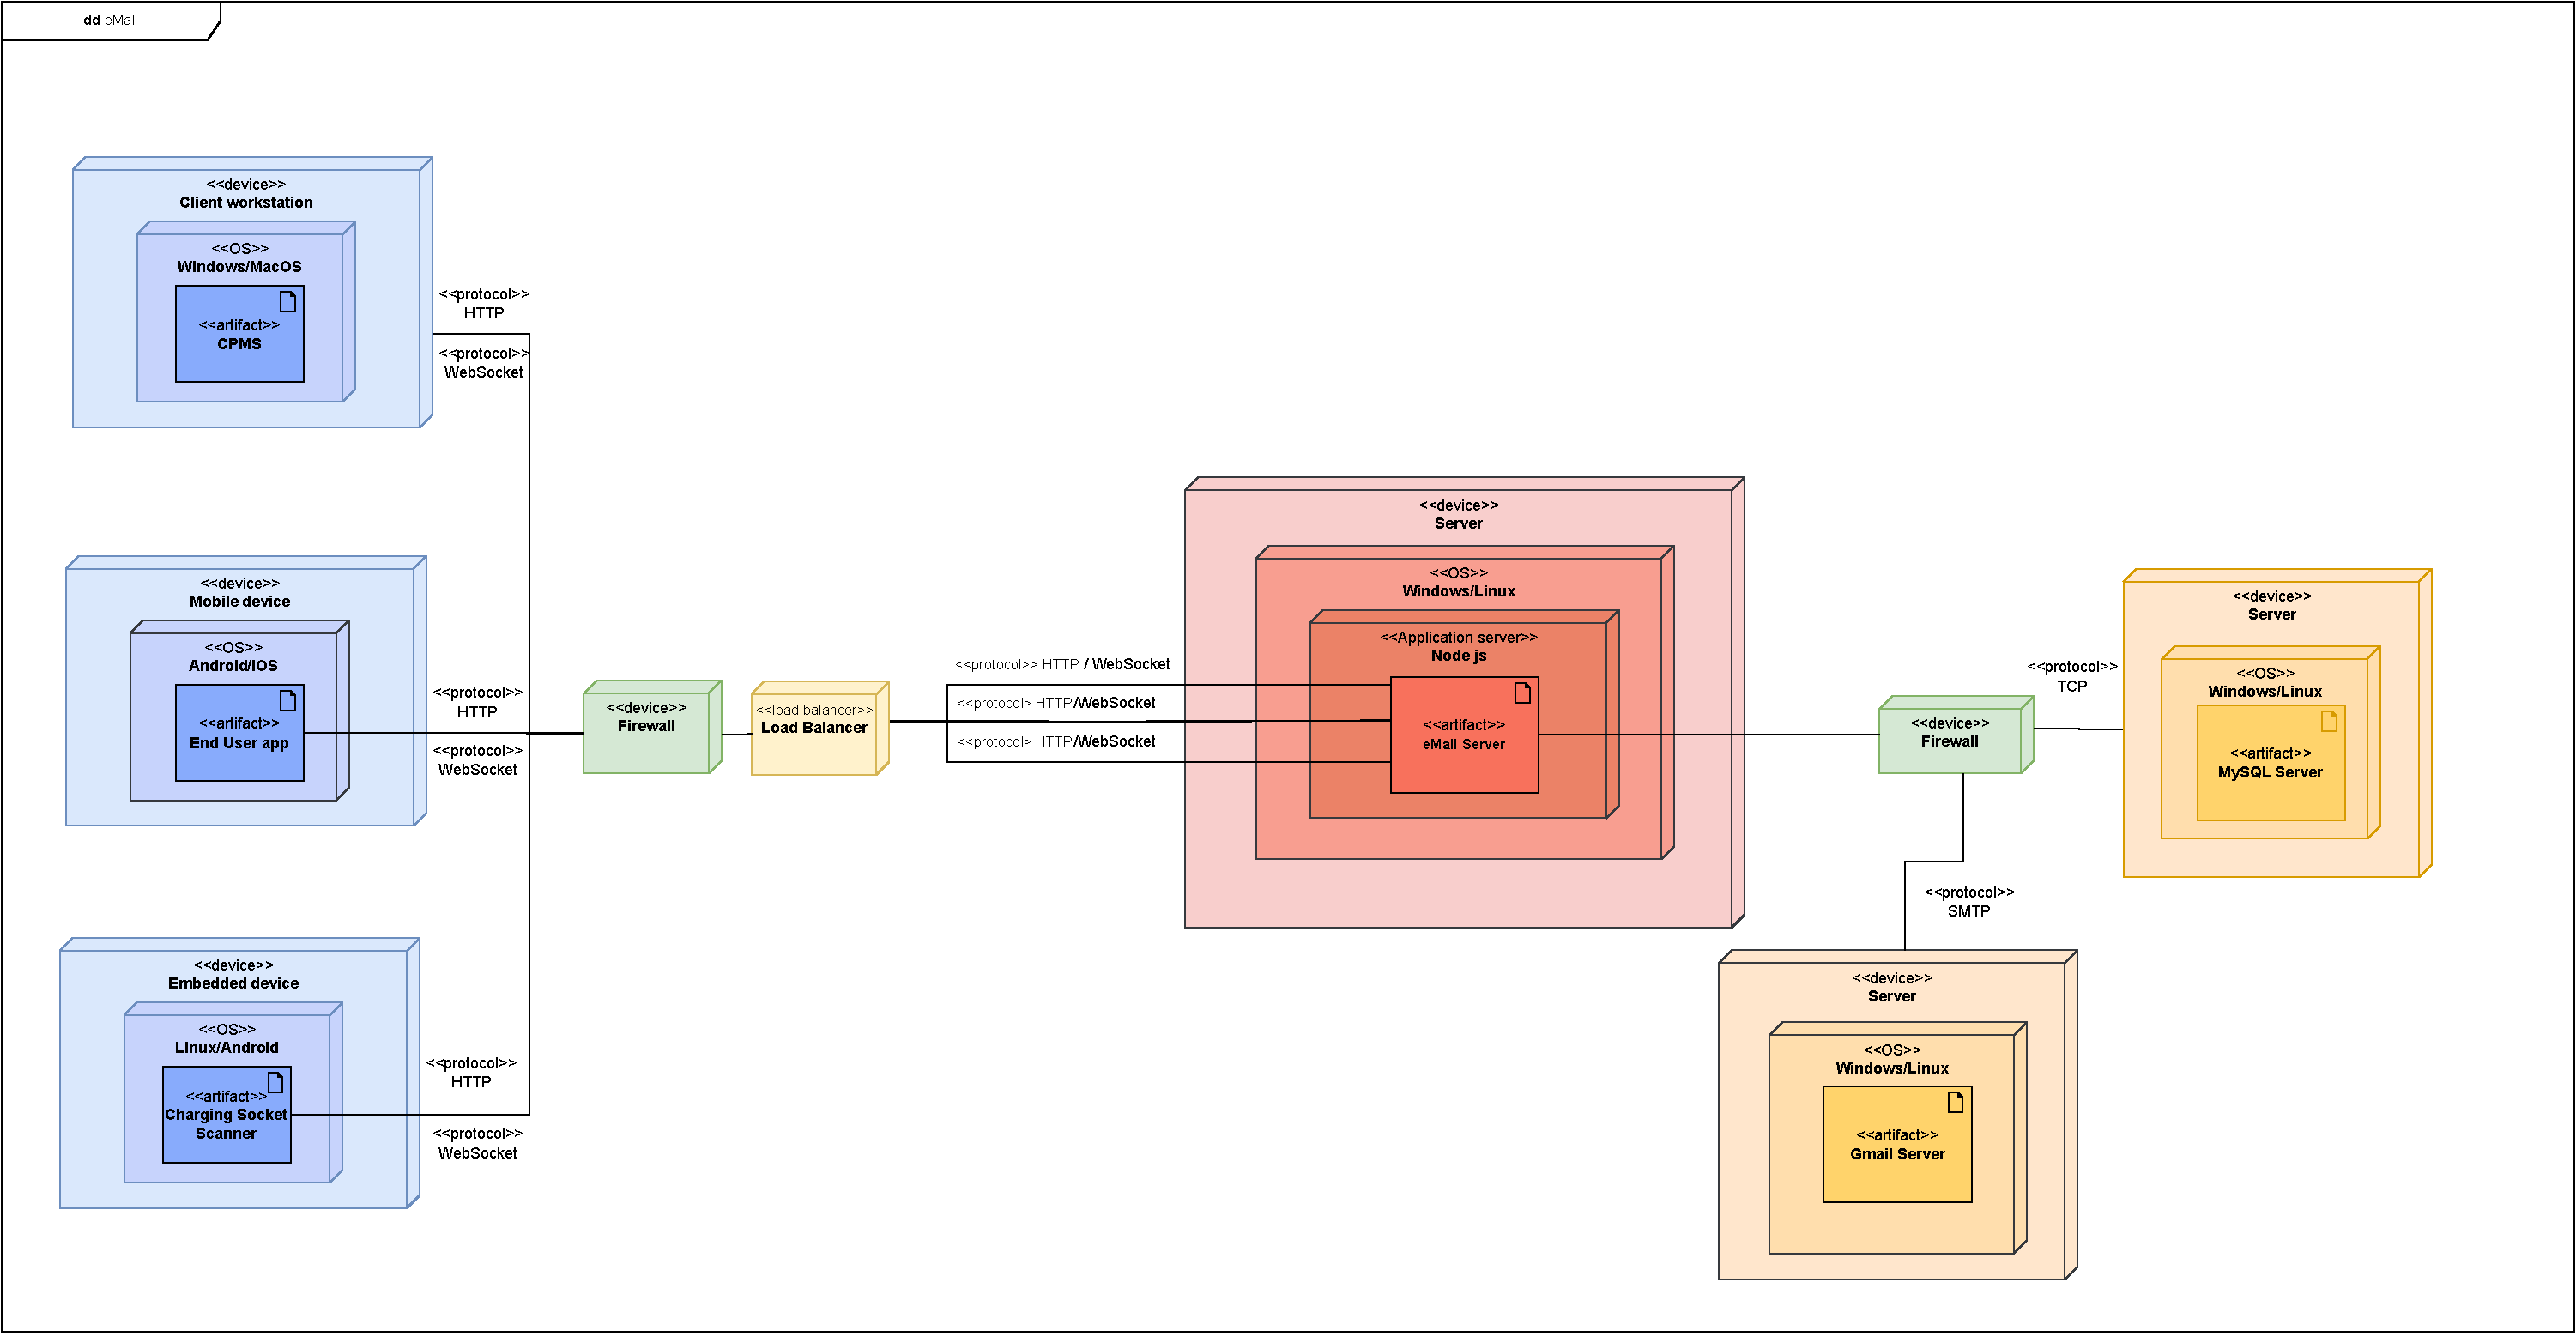
\includegraphics[width=\textwidth]{images/deployment.pdf}
    \caption{Deployment Diagram eMall system.}
    \label{fig:deployment_diagram}
\end{figure}
As shown in the figure \ref{fig:deployment_diagram} above, the architecture of the system is composed of \textbf{3-tiers}.\\
Also the presence of non-logical elements are useful to ensure a lot of benefits in the whole system:
\begin{itemize}
    \item \textbf{Firewalls}: network security device which monitors all incoming and outgoing traffic and based on a defined set of security rules it accepts, rejects or drops that specific traffic. It allows to have greater security in the whole system.
    \item \textbf{Load Balancer}: A load balancing system acts as a single point of contact for clients. The load balancing system automatically distributes incoming traffic between multiple destinations. This increases the availability of the application in case of a lot of connections.
\end{itemize}
In the following, each tier is meticulously analysed:
\begin{itemize}
    \item \textbf{Presentation tier}: It's the front-end of the application and concerns everything to do with graphics for users. It's the user interface and communication layer of the application, where the end user interacts with the application: this top-level tier can run on a web browser, as desktop application or as a mobile application. In particular:
    \begin{itemize}
        \item \textit{End User app}: It's installed on the user's mobile device and is compatible with Android and iOS. It communicates with the application tier through HTTP.
        \item \textit{CPMS}: It's a web application that runs on modern browsers (e.g. Mozilla Firefox, Google Chrome) and communicates with the application tier always via HTTP.
        \item \textit{Charging Socket Scanner}: It's an application installed exclusively on the charging socket in order to scan the code of a user's booking. It communicates with the application tier sending data related to the charging socket.
    \end{itemize}
    \item \textbf{Application tier}: It's the system's application server and it's the heart of the application. It contains all the logic that is executed on multiple instances of NodeJS.\\
    In this tier, information collected in the presentation tier is processed and managed: moreover this tier is able to add, delete or modify data in the data tier. It also communicates with the dedicated mail server via the SMTP protocol.
    \item \textbf{Data tier}: consists of the DBMS server that uses MySQL to store data processed by the application in tabular form (relational database).  
\end{itemize}
\section{Runtime view}
This section describes the most important components interactions of the system.
For the sake of simplicity the sequence diagrams are based on the first level of components.
\subsection{End user app login}
At the beginning the end user must log in to use the main functions of the application. The login is done by entering the username and password, if the credentials are present in the database the process will be successful and he will be able to use the application, otherwise he will have to repeat the procedure.
\begin{figure}[H]
    \centering
    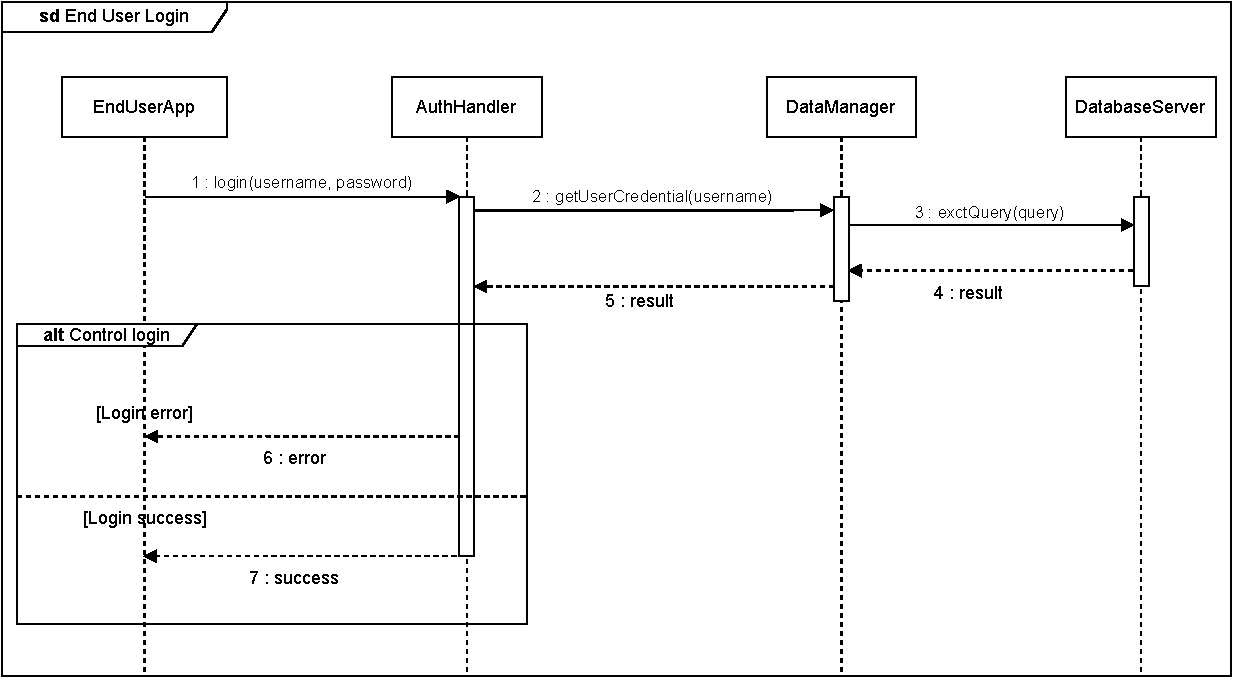
\includegraphics[width=\textwidth]{images/sd_endUserLogin.pdf}
    \caption{End User Login sequence diagram}
    \label{fig:endUserLogin}
\end{figure}
\subsection{CPO app login}
In this case the login is the same as the one seen previously, the only difference is that the credentials are entered by a CPO and access to a different system.
\begin{figure}[H]
    \centering
    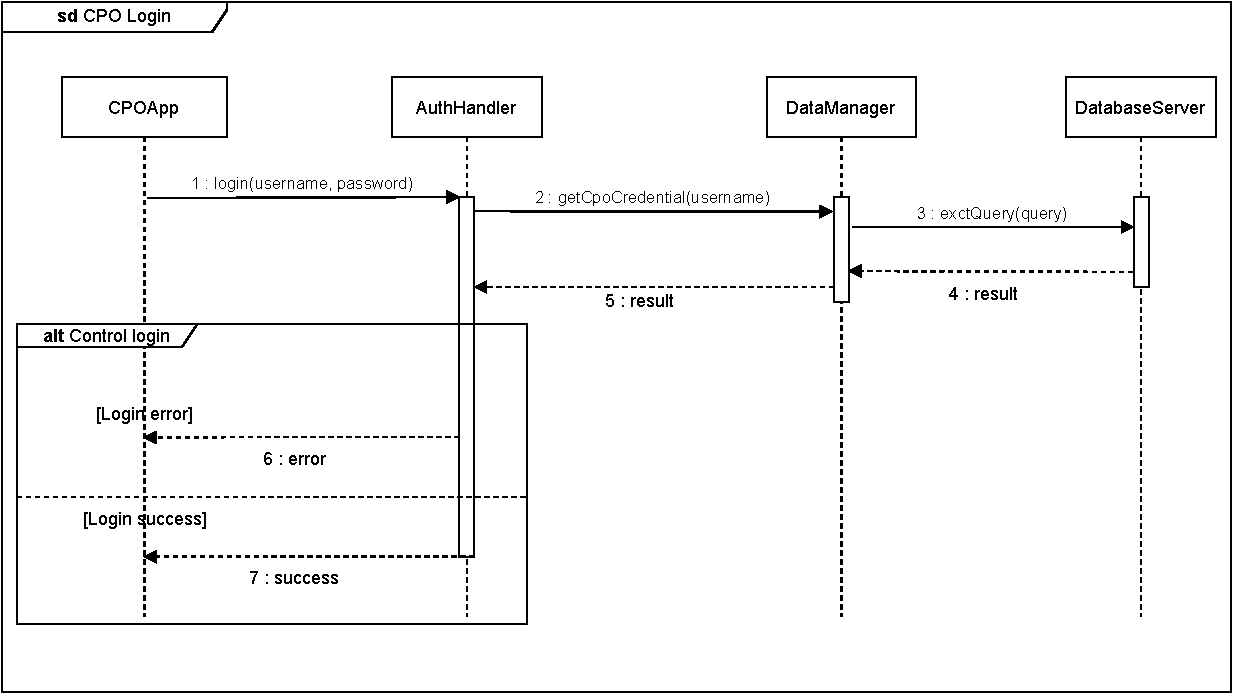
\includegraphics[width=\textwidth]{images/sd_cpoLogin.pdf}
    \caption{CPO Login sequence diagram}
    \label{fig:endUserLogin}
\end{figure}
\subsection{Make a booking}
The following sequence diagram is used to explain how to make a reservation. The end user from his application can create a reservation, which is sent to the database. Within the database it is verified that those data are not already present, if so the reservation is confirmed while otherwise it is denied. If the booking is confirmed, a unique QR-Code is generated.
\begin{figure}[H]
    \centering
    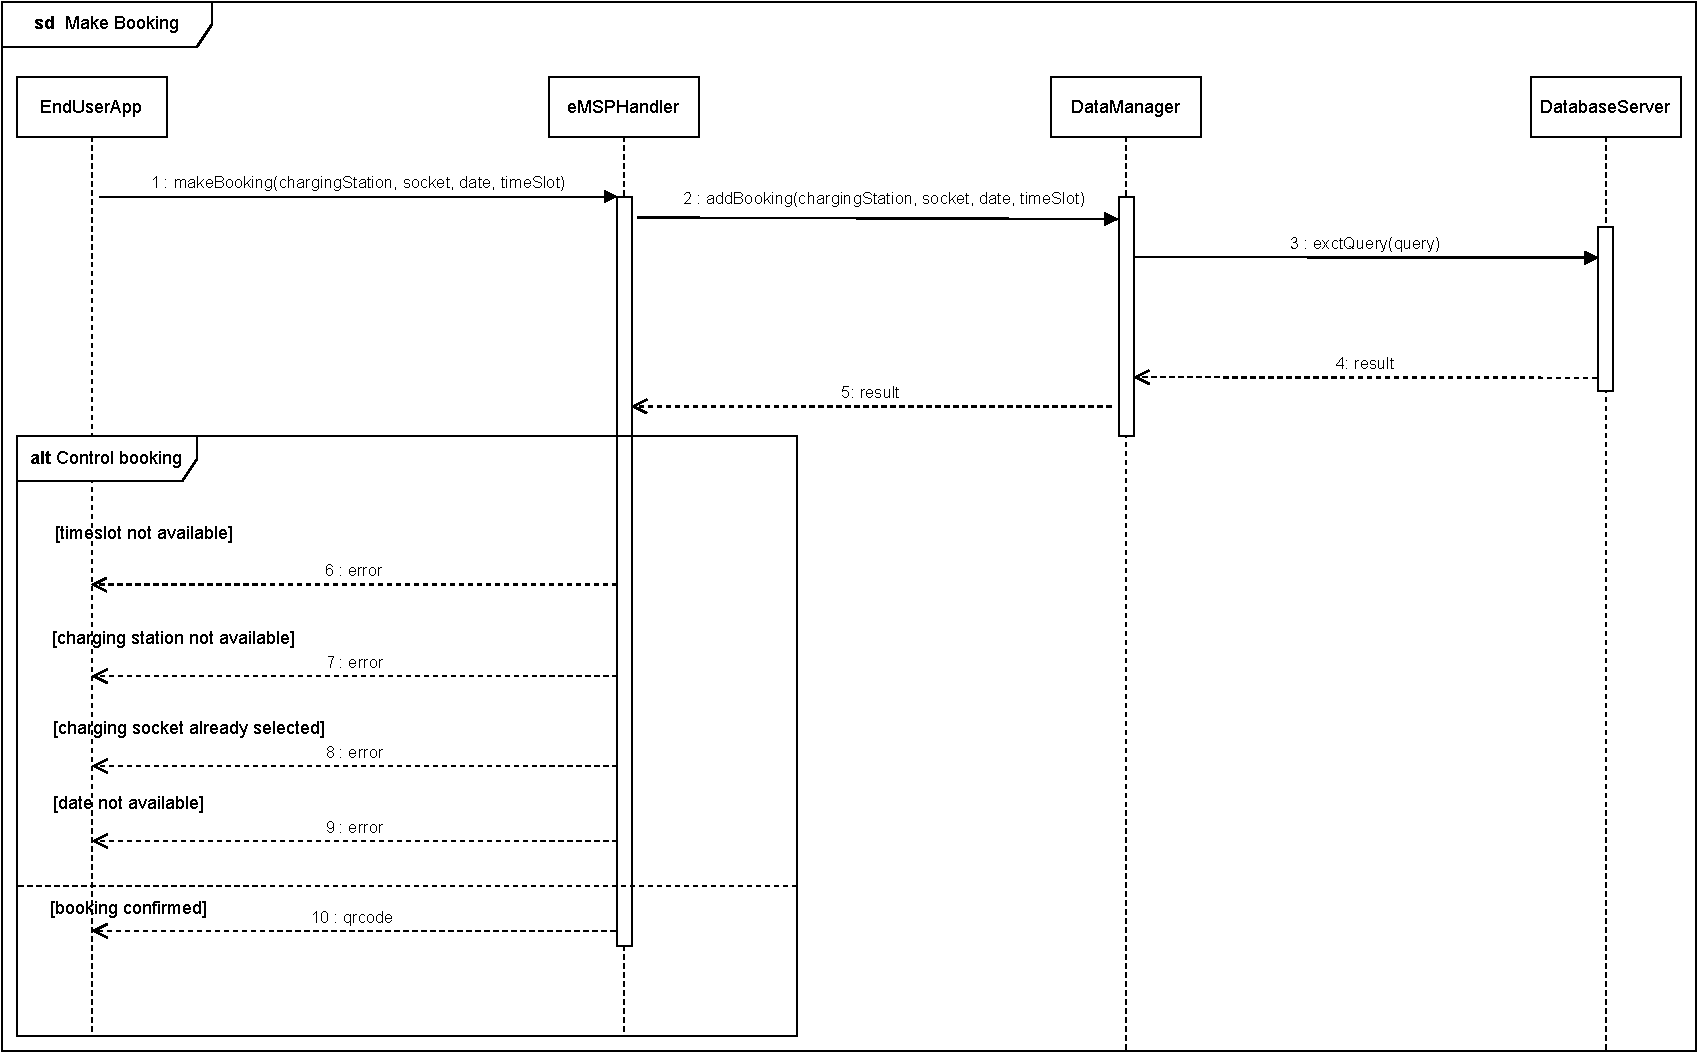
\includegraphics[width=\textwidth]{images/sd_bookingRequest.pdf}
    \caption{Make a booking sequence diagram}
    \label{fig:makeBooking}
\end{figure}
\subsection{Check QR-Code}
The socket is used to check, through a scanner, the QR-Code of the pronotation. Through this scan, the QR-Code is associated with the reservation and by communicating with the database, it verifies that the reservation is associated with the correct QR-Code.
\begin{figure}[H]
    \centering
    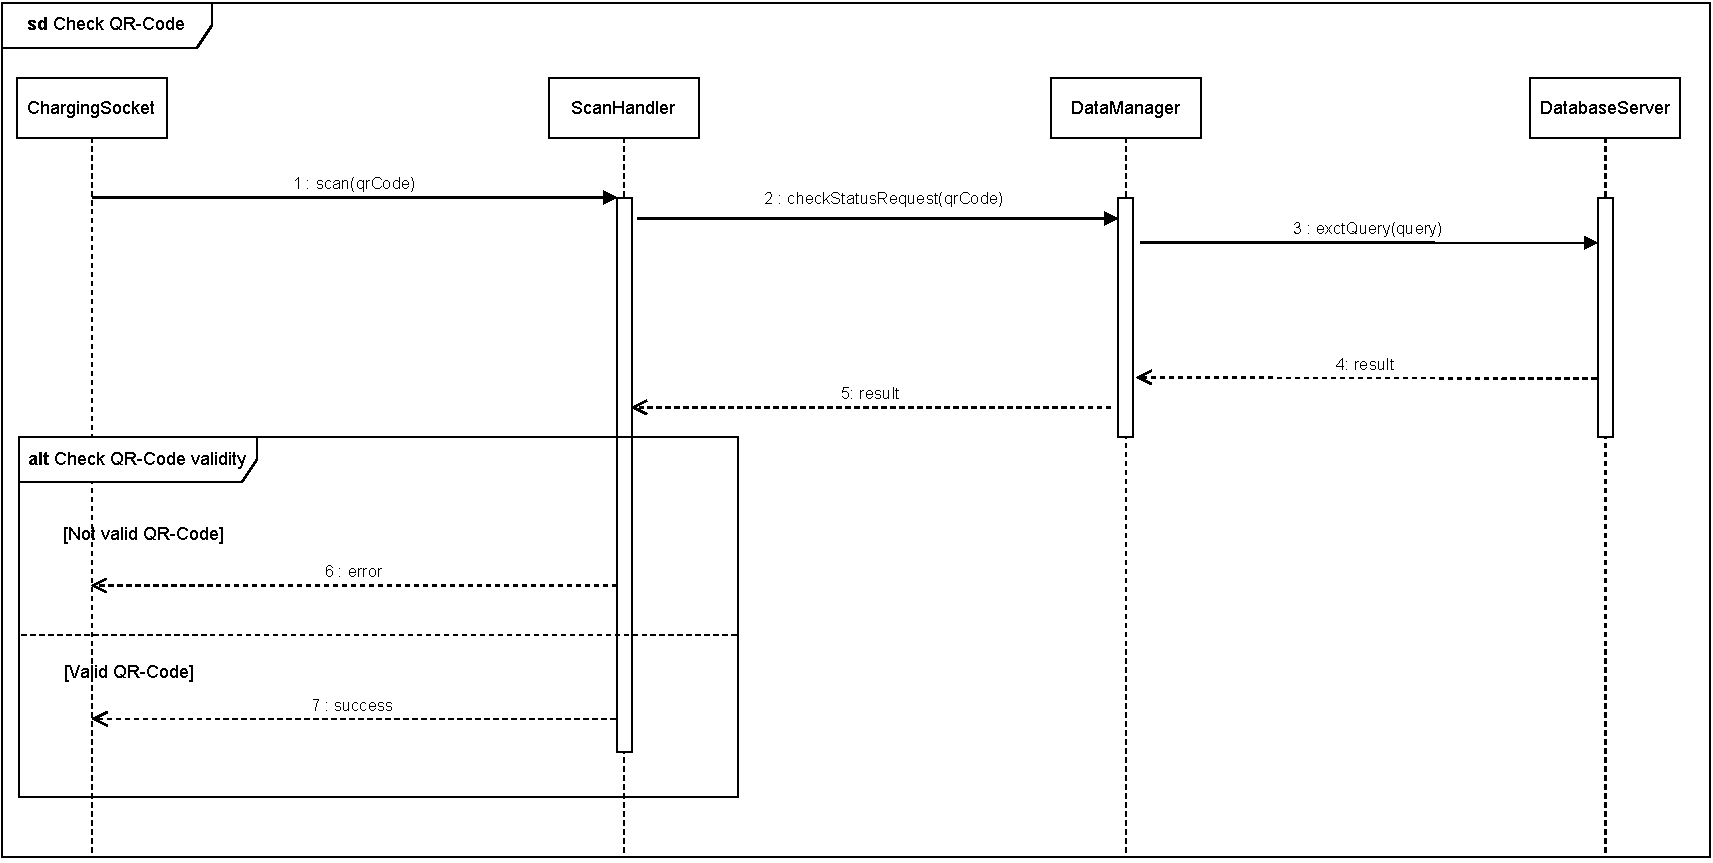
\includegraphics[width=\textwidth]{images/sd_qrCodeScan.pdf}
    \caption{QR-Code scan sequence diagram}
    \label{fig:qrCodeScan}
\end{figure}
\subsection{Charging station registration}
The charging station registration is performed by a CPO via the web app after his login. Prompted
information are checked from the system and then, if the charging station doesn’t already exist, the
charging station is saved into the database.
\begin{figure}[H]
    \centering
    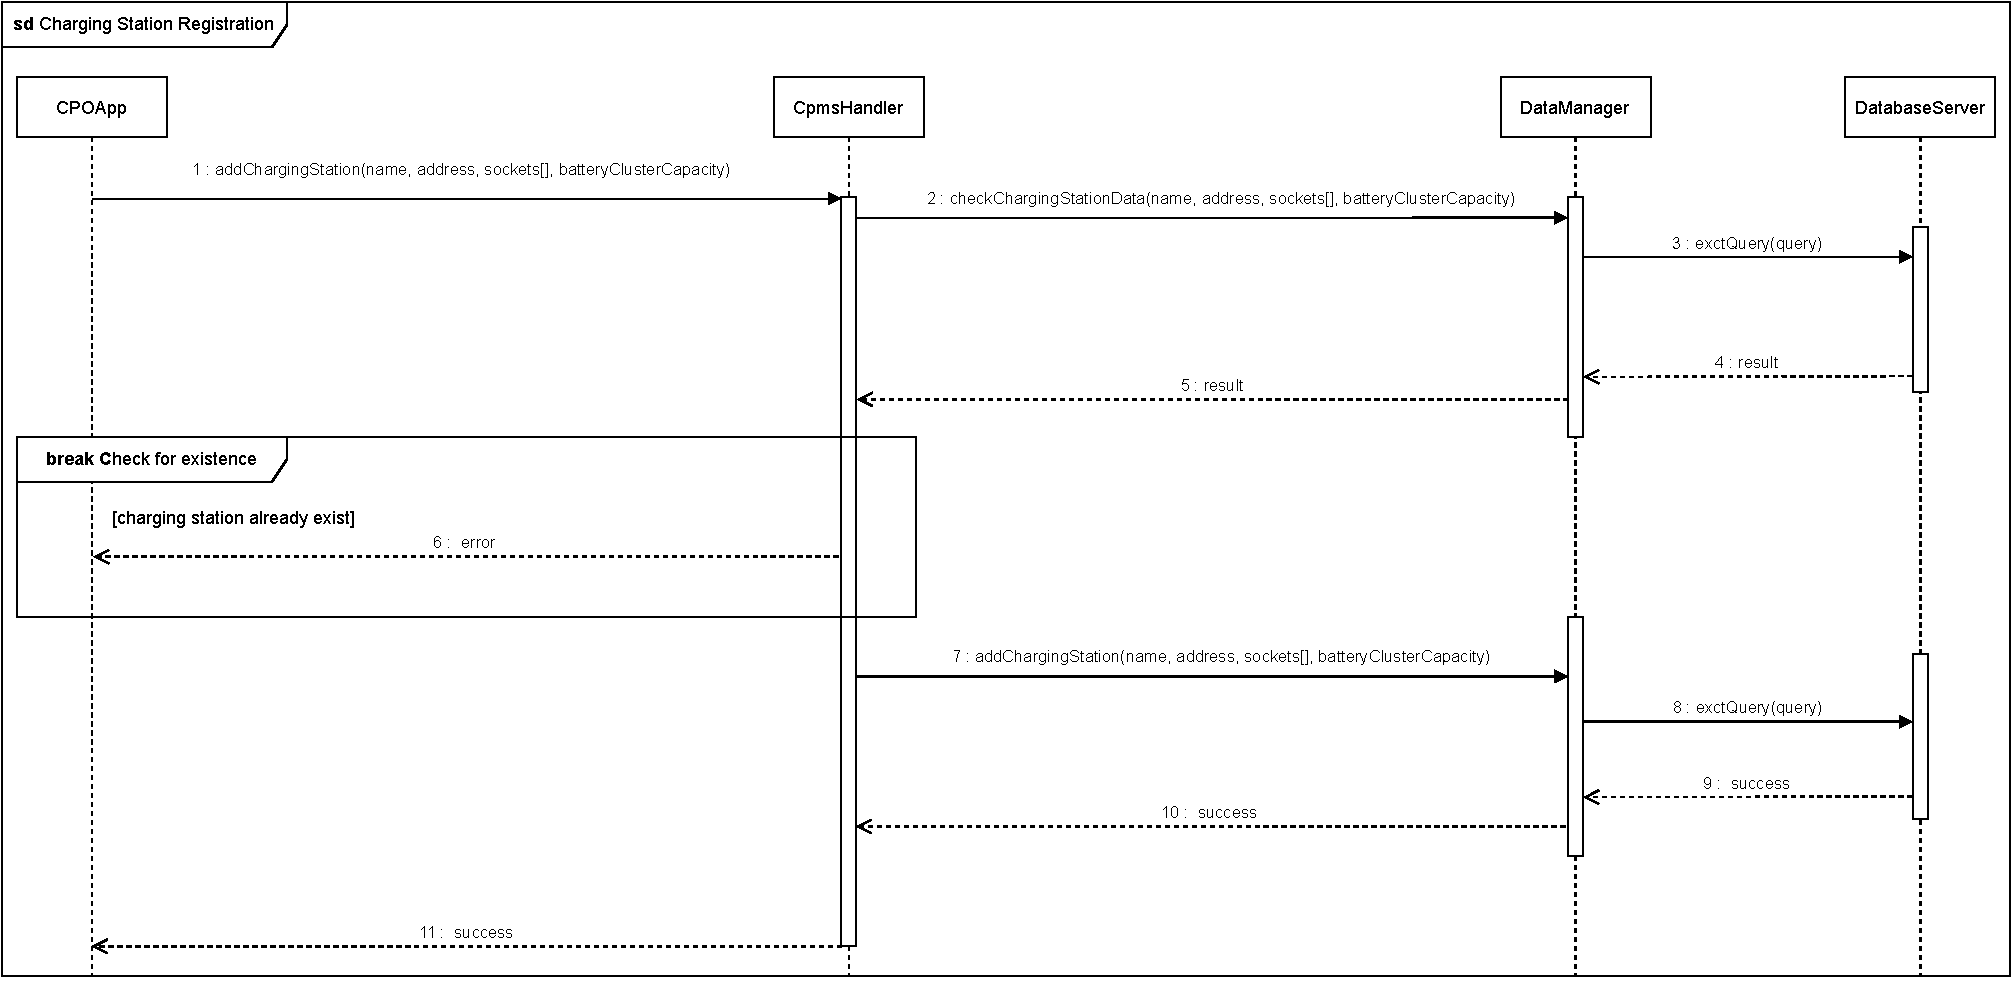
\includegraphics[width=\textwidth]{images/sd_chargingStationRegistration.pdf}
    \caption{Charging station registration sequence diagram}
    \label{fig:chargingStationRegistration}
\end{figure}
\subsection{End User Payment}
The following sequence diagram is used to describe how money is withdrawn from the user's cards after using the vehicle top-up service. First of all, it is verified that the payment method and its data are correct through the database; after that, it is verified that there is sufficient credit to pay the requested sum and if there is, the payment receipt is sent via email.
\begin{figure}[H]
    \centering
    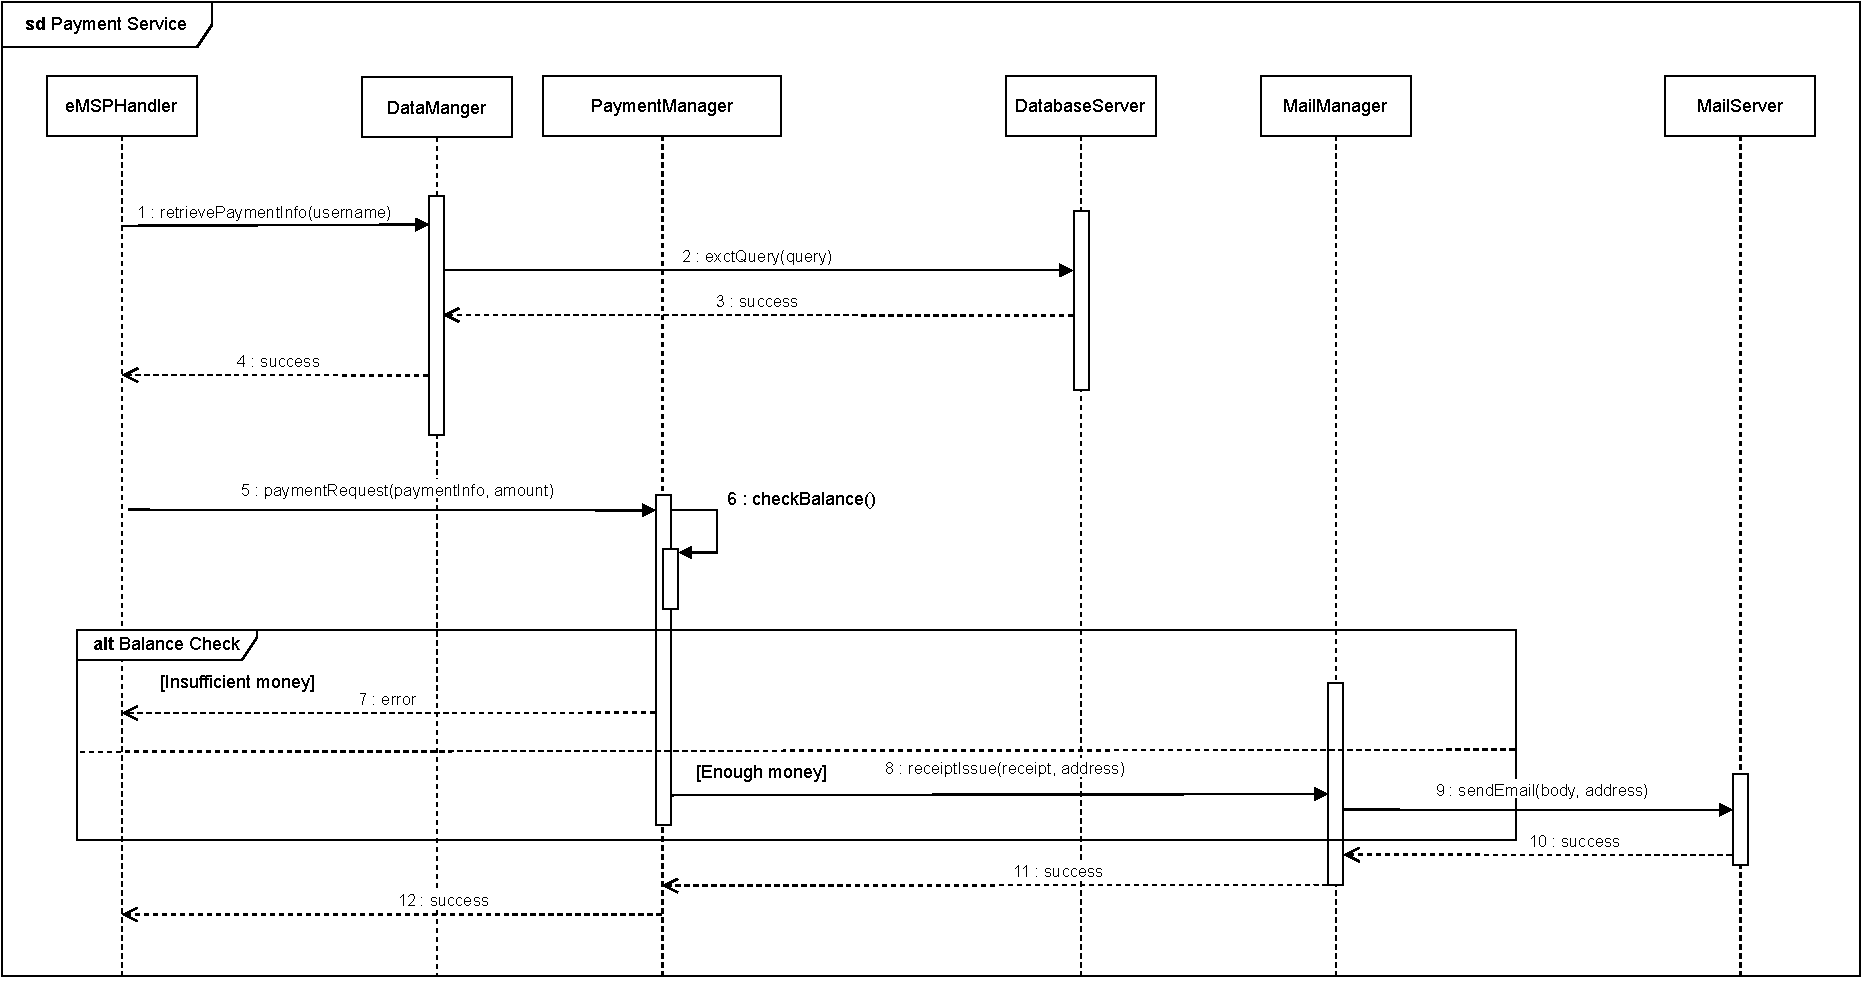
\includegraphics[width=\textwidth]{images/sd_paymentMethod.pdf}
    \caption{End User Payment sequence diagram}
    \label{fig:endUserPayment}
\end{figure}
\subsection{DSO Interaction}
The interaction with DSO is performed by a CPO via the web app after his login. Through the web app, the CPO is able to view the list of energy offers presented by the various DSOs. Furthermore, thanks to the payment method external to the system for CPOs, they can buy energy from the DSOs simply by selecting the offer that most convinces them.
\begin{figure}[H]
    \centering
    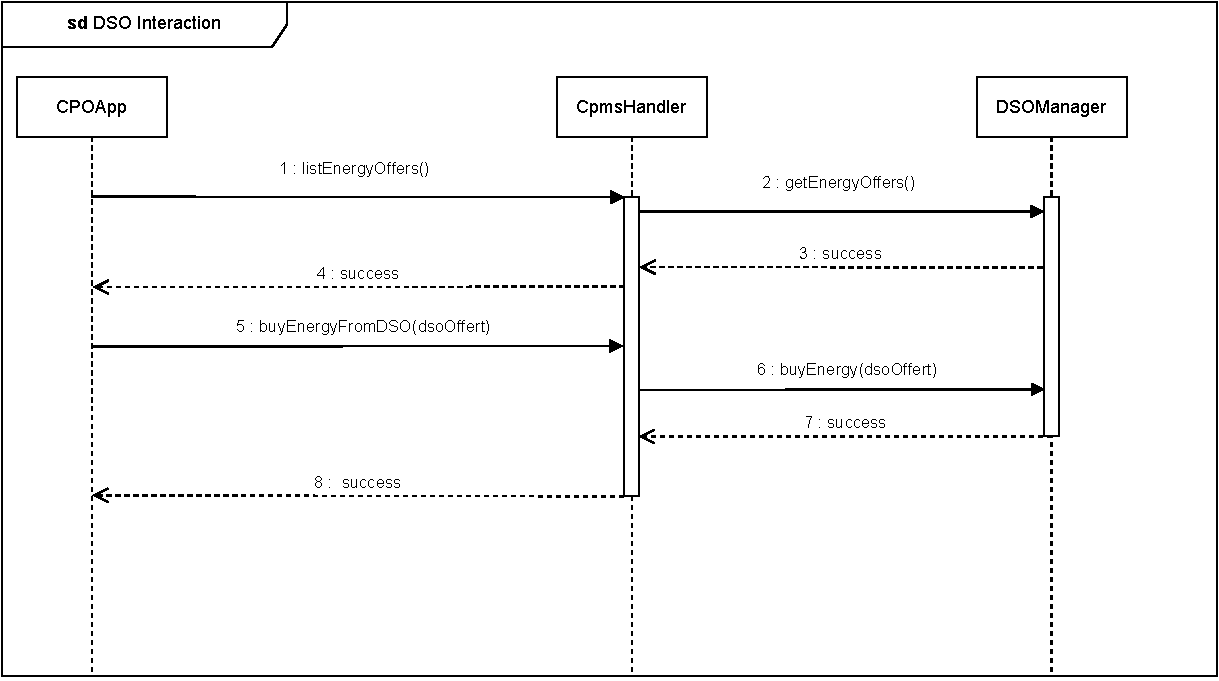
\includegraphics[width=\textwidth]{images/sd_DSO.pdf}
    \caption{DSO Interaction sequence diagram}
    \label{fig:endUserPayment}
\end{figure}
\subsection{Check charging socket's status}
The following sequence diagram is used to describe how sockets are checked to be busy or not. To do this it is necessary to send a request to the database regarding the status of a given socket, it is able to tell if the socket is free for use or not via a "status" flag.
\begin{figure}[H]
    \centering
    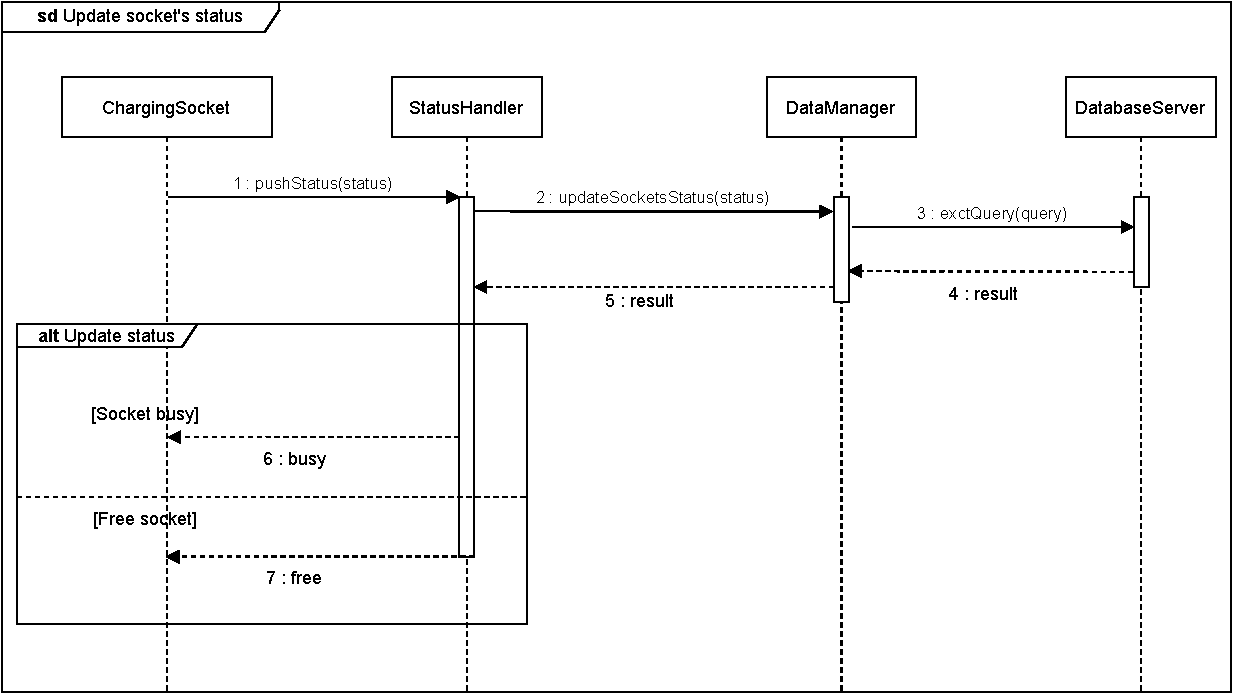
\includegraphics[width=\textwidth]{images/sd_status.pdf}
    \caption{Check status sequence diagram}
    \label{fig:checkStatus}
\end{figure}
\section{Component interfaces}
\begin{figure}[H]
    \centering
    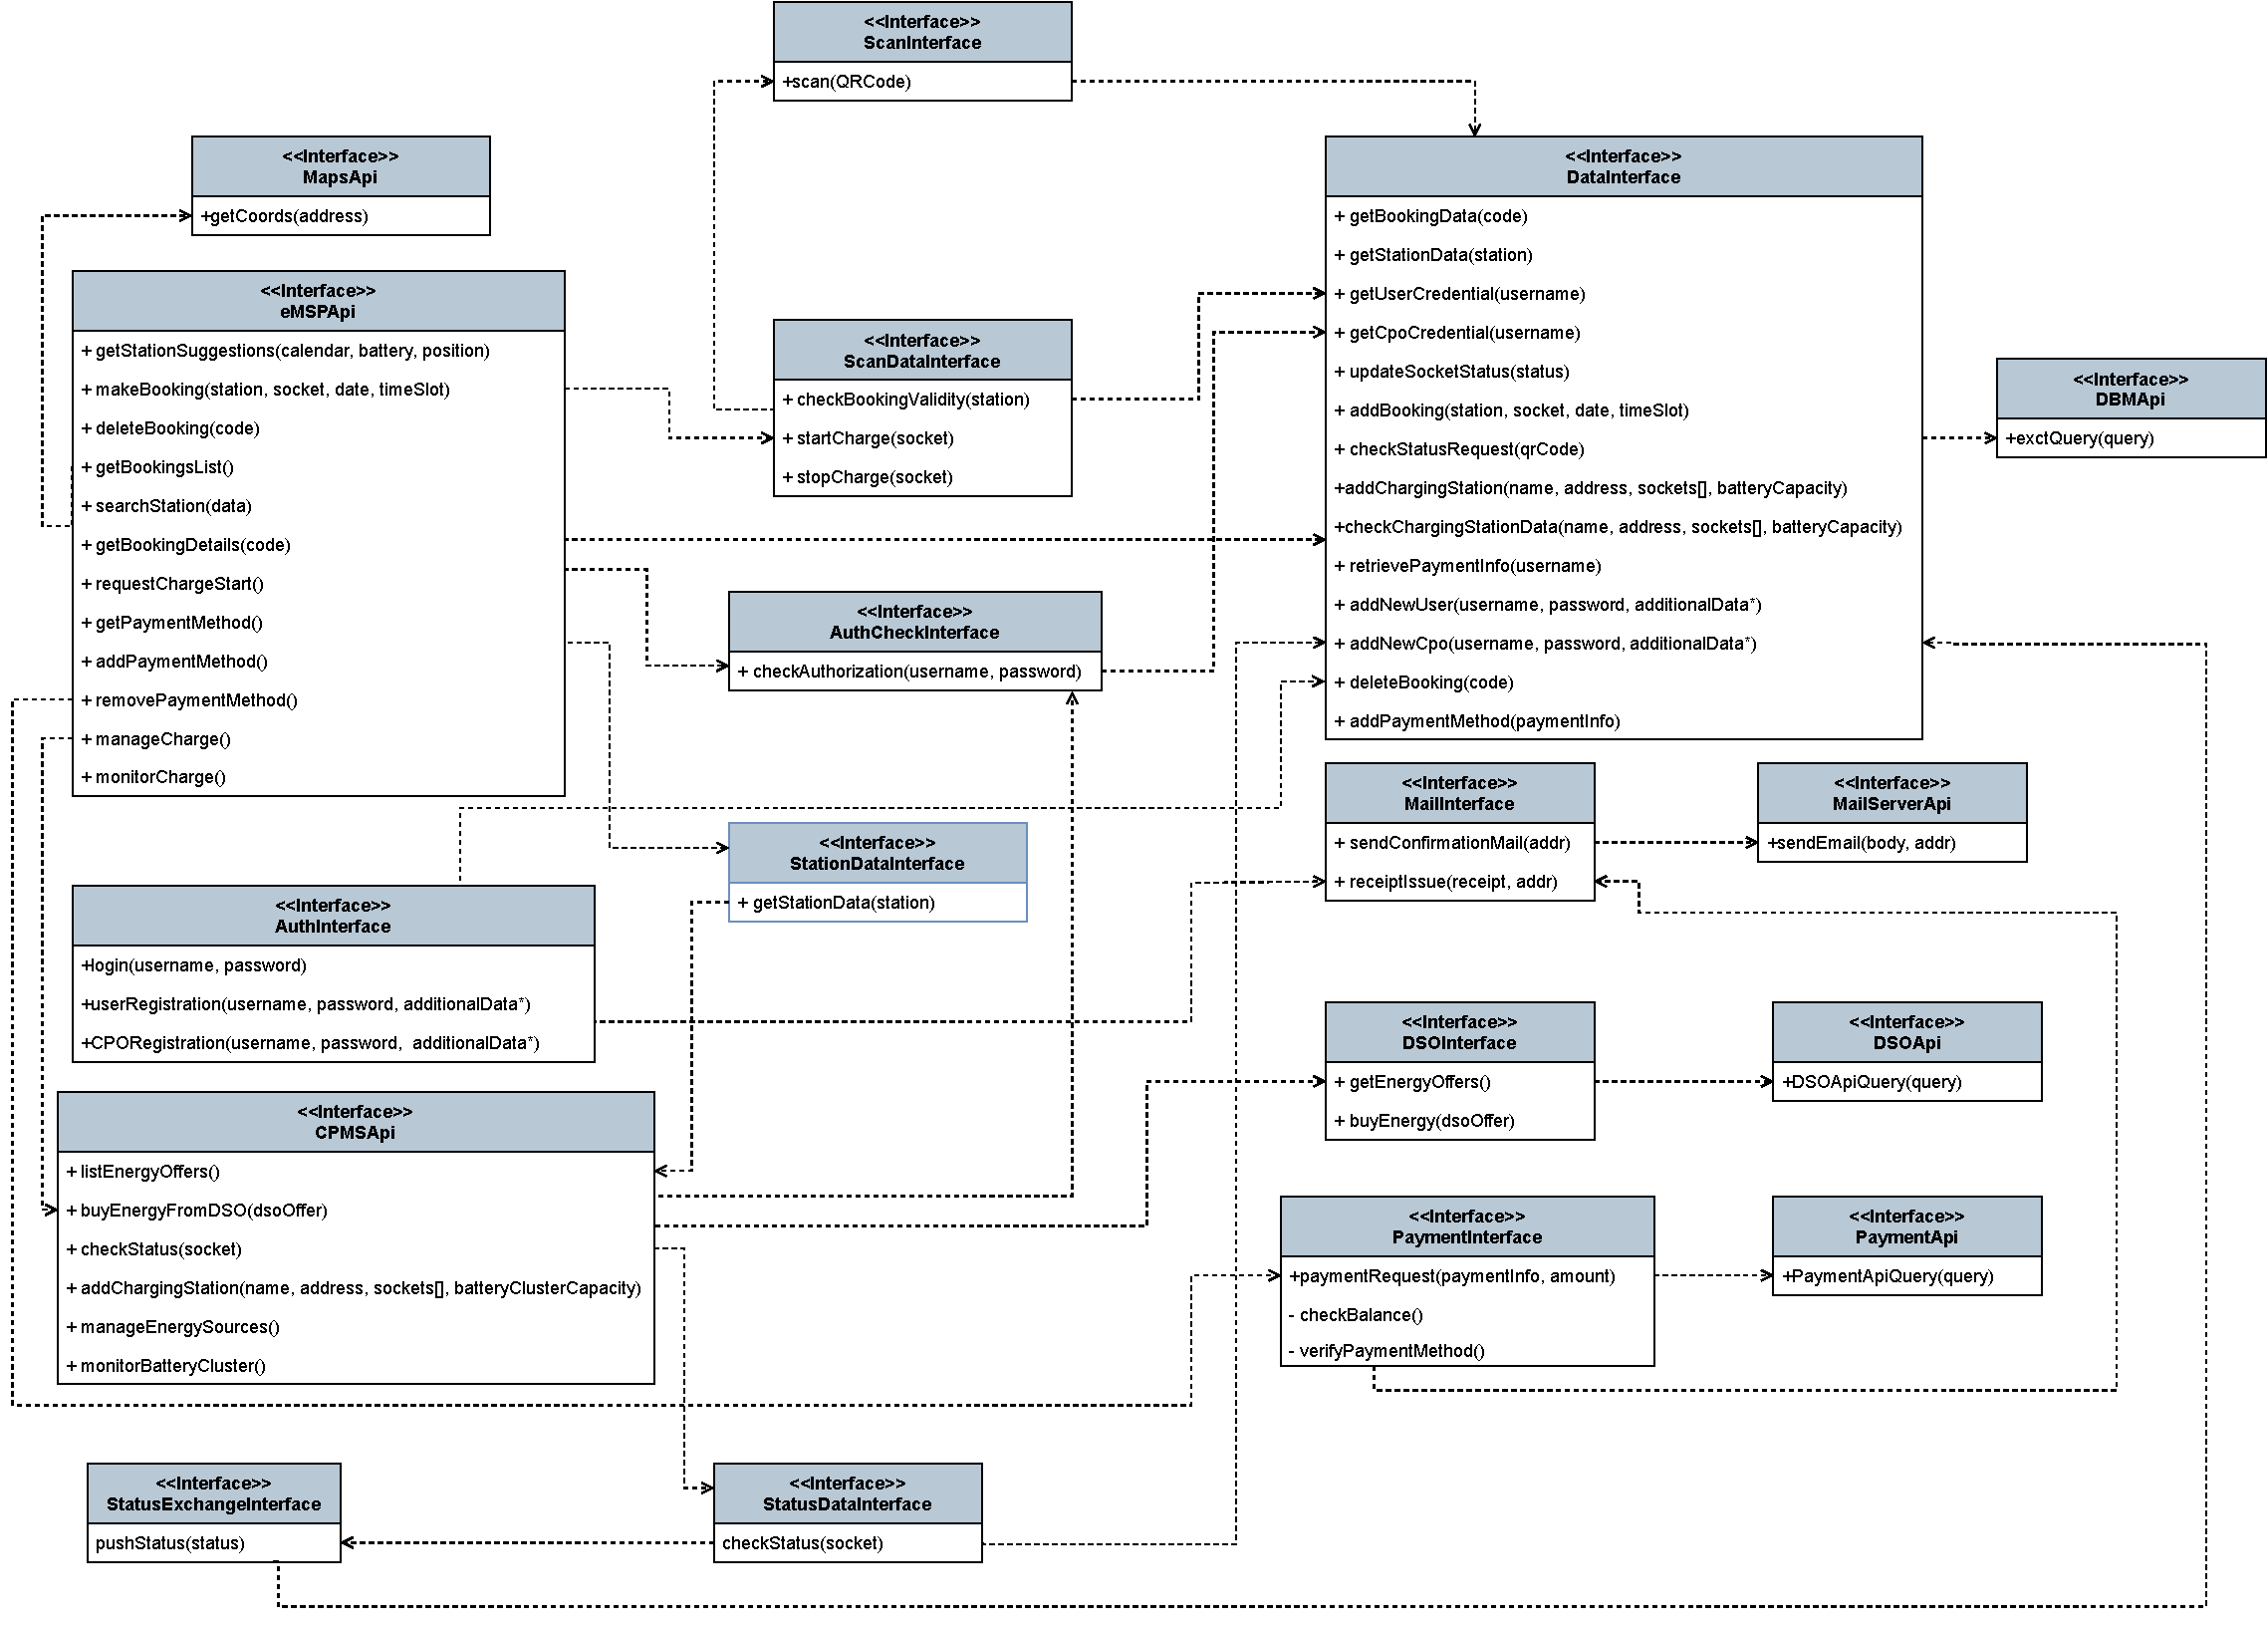
\includegraphics[width=\textwidth]{images/InterfaceDiagram.pdf}
    \caption{Interface diagram.}
    \label{fig:interface}
\end{figure}
\section{Selected architectural styles and patterns}
In this section, the architectural styles and patterns of the eMall system will be analysed.
\begin{itemize}
    \item \textbf{3-tiers architecture}: eMall system, as illustrated before, is composed by 3 tiers: presentation tier, application tier and data tier.\\
    This architectural choice is due to the fact that the macro roles of the system are separated as much as possible, favouring the quality of each component. Indeed, the most important features of this architecture it's logical and physical separation of functionality: each tier can run on a separate operating system and server platform and runs on at least one dedicated server hardware or virtual server, so the services of each tier can be customized and optimized without impact the other tiers. 
    Furthermore, below are shown some 3-tiers architecture benefits:
\begin{itemize}
    \item \textbf{Faster development}
    \item \textbf{Improved scalability}
    \item \textbf{Improved reliability}
    \item \textbf{Improved security}
\end{itemize}
\begin{figure}[H]
    \centering
    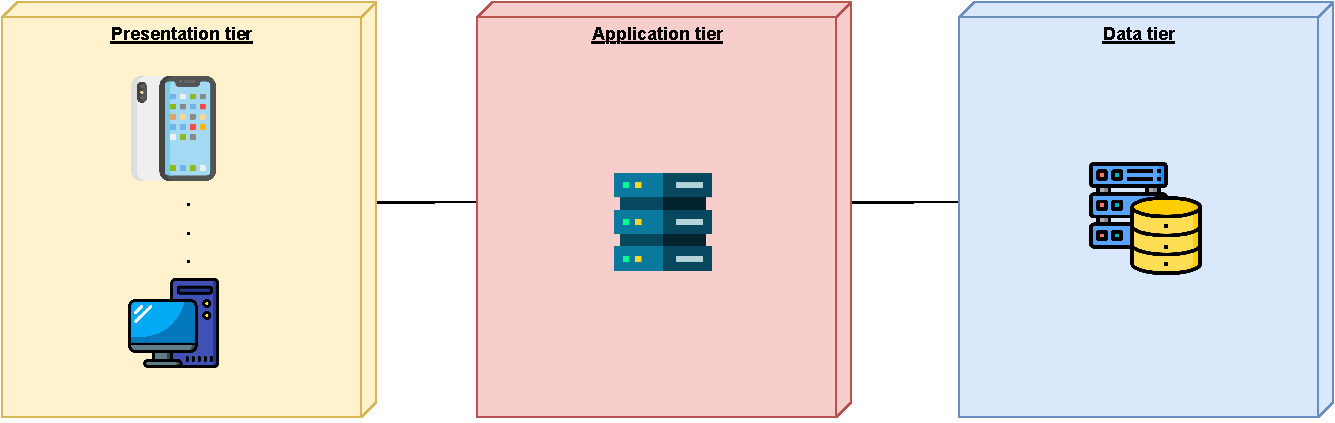
\includegraphics[width=0.8\textwidth]{images/3tier_shape.pdf}
    \caption{3-tier architecture}
    \label{fig:3-tier}
\end{figure}
\item \textbf{RESTful APIs}: RESTful API is an interface that two computer systems use to exchange information securely over the internet. In the eMall system are used to exchange object and information in JSON format through HTTP. 
\item \textbf{Model View Controller}: Model-View-Controller (MVC) is a software architecture model. Provides an architecture consisting of three different parts: data (Model), data visualisation (View) and input management (Controller).\\
These three components are interconnected: the Model is shown via the View to the user, who produces the input with which the Controller updates the Model. 
\begin{figure}[H]
    \centering
    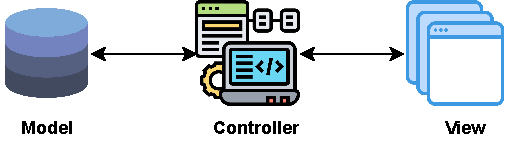
\includegraphics[width=0.8\textwidth]{images/restful_api.pdf}
    \caption{Model View Controller pattern}
    \label{fig:mvc}
\end{figure}
\end{itemize}
\section{Other design decision}
\subsection{Real time communication}
The interaction between CPMS, eMSP, the charging socket and the eMall server, for some tasks need to be real time, to do this the WebSocket protocol is used. 
\subsection{Maps APIs}
The eMall system has to provide a service that allows the end user to visualize himself on the map and the nearby charging station. To achieve this goal is necessary to use specifics maps APIs that retrieve these information.
\subsection{Database structure}
\textit{In the below figures is important to note that in order to simulate the interaction between CPOs and DSOs about the purchasing of energy, has been created a DSO table on database.\\
That is, obviously, a simplified choice given an absence of external DSOs APIs.}
\subsubsection{ER diagram}
\begin{figure}[H]
    \centering
    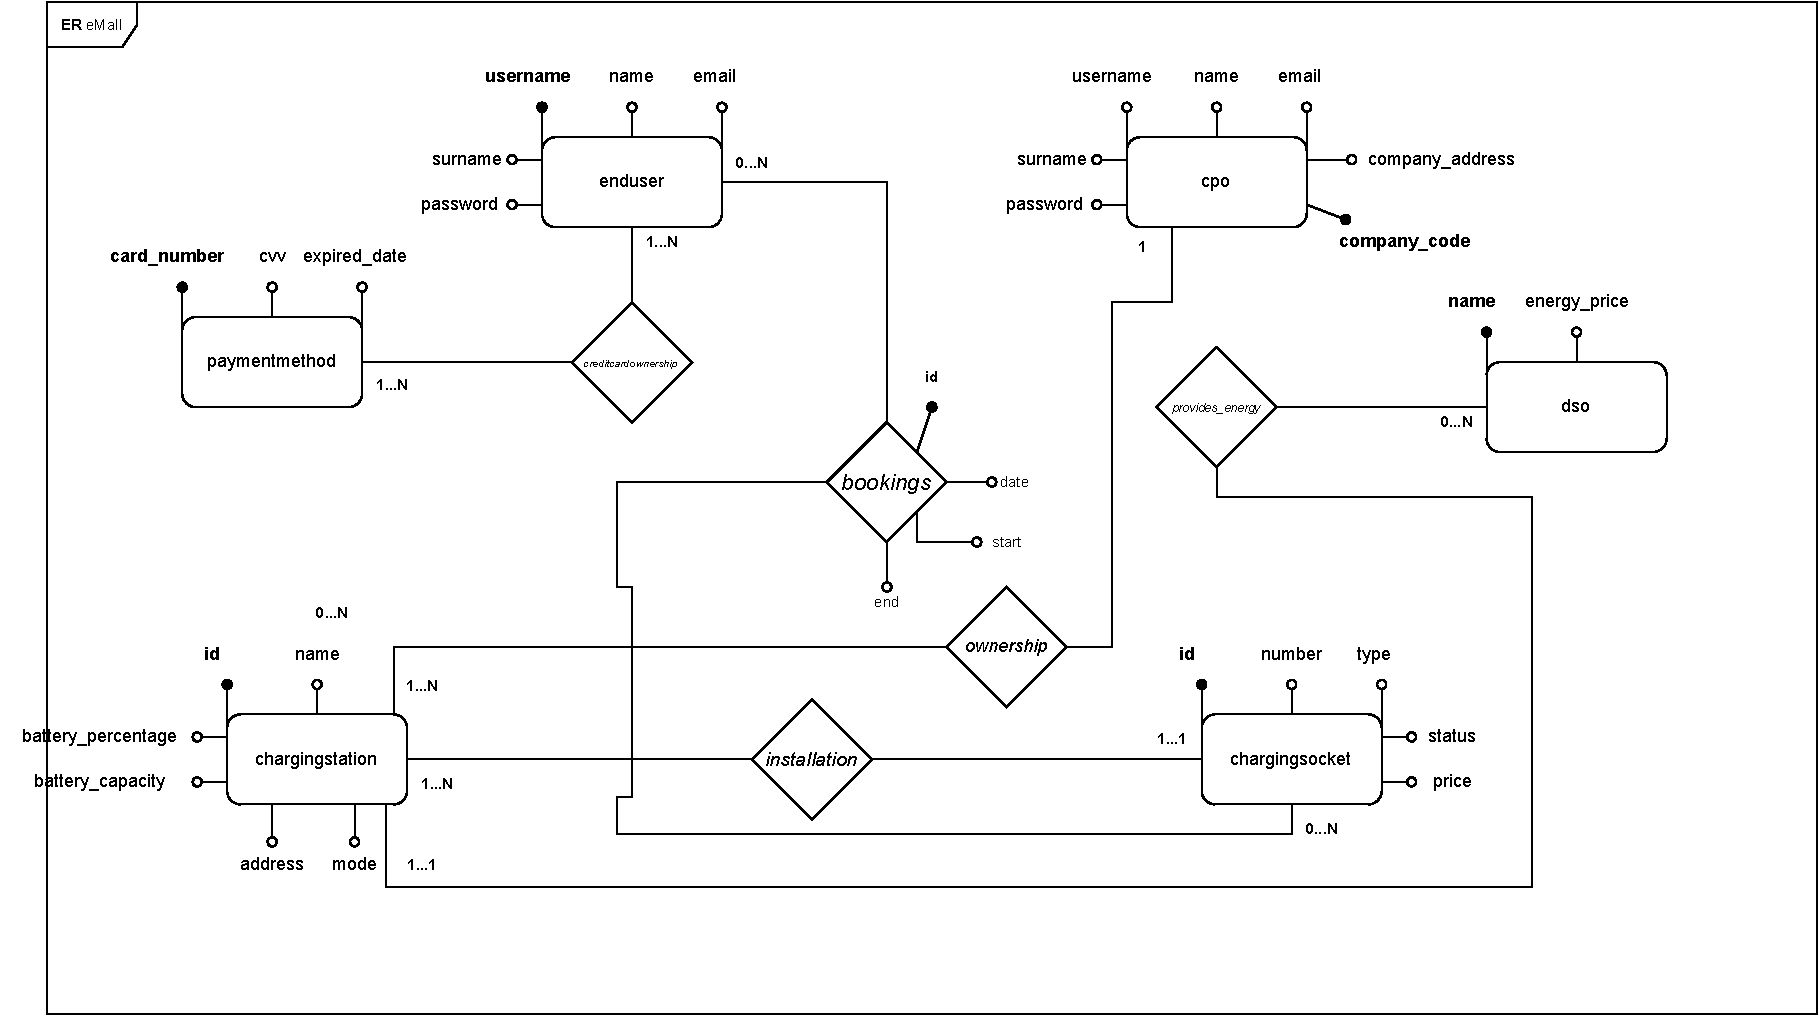
\includegraphics[width=0.8\textwidth]{images/er_db.pdf}
    \caption{Entity-Relation diagram of eMall database}
    \label{fig:er_diagram}
\end{figure}
\subsubsection{Relational schema}
\begin{figure}[H]
    \centering
    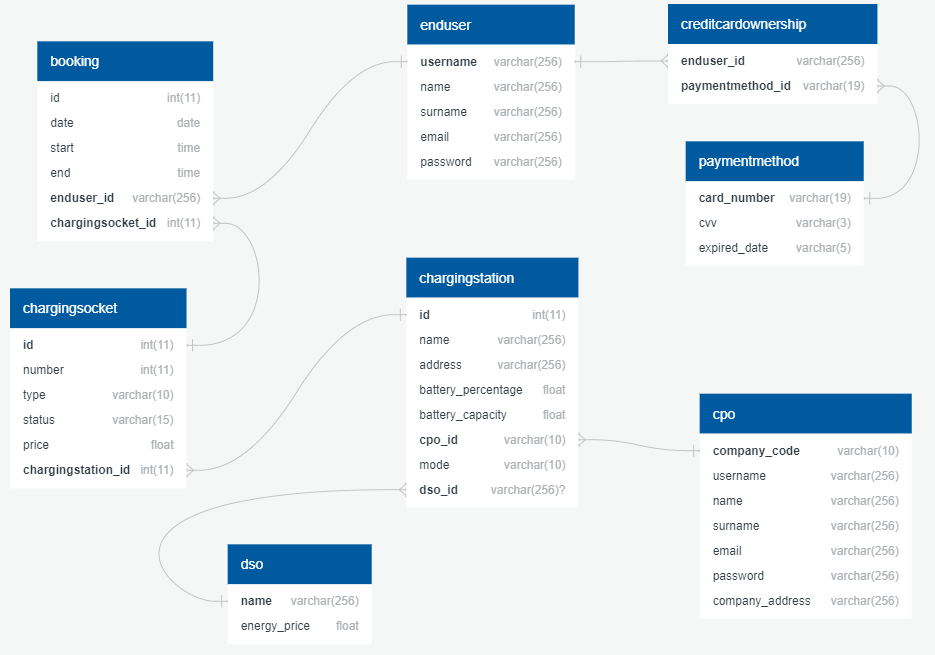
\includegraphics[width=0.8\textwidth]{images/db_structure.png}
    \caption{Relational schema of eMall database}
    \label{fig:dbstructure}
\end{figure}
